\section{Theorie}

\subsection{Elektronenkanone}
Ein Elektronenstrahl wird i.A., so auch bei diesem Experiment, mithilfe einer Glühkathode in Kombination mit einem Wehneltzylinder
erzeugt. Dieser Aufbau wird auch Elektronenkanone genannt.\\
Zuerst wird eine sogenannte Heizspule (Glühkathode) mit der Heizspannung $U_H$ zum Glühen gebracht. Die dadurch freigesetzten Elektronen werden in einer
Zylinderkathode (Wehneltzylinder) auf den Mittelpunkt dieser fokussiert und dann durch eine Anodenplatte mit einem kleinen Loch in der Mitte beschleunigt, da auf der Anode eine Potentialdifferenz $U$ gegenüber der Kathode herrscht.\\
\begin{figure}[!htbp]
\centering
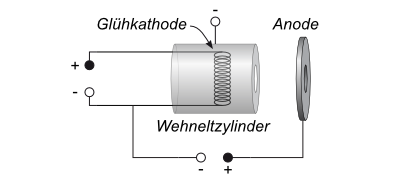
\includegraphics[scale = 0.9]{elektronenkanone.png}
\caption{Aufbau einer Elektronenkanone} \label{elektronenkanone}
\end{figure} \newline
Die durch Spannung hervorgerufene Energie $E=e\*U$ entspricht relativ genau der kinetischen Energie der Elektronen $e$. Damit gilt für die Geschwindigkeit $v$ eines Elektrons der Masse $m_e$:
\begin{align}
e\*U&=E_{kin_{e}}=\frac{1}{2}m_ev^2 \\
v&=\sqrt{\frac{2eU}{m_e}} \label{kanone}
\end{align}

\subsection{Helmholtzspule}

\begin{figure}[!htbp]
\centering
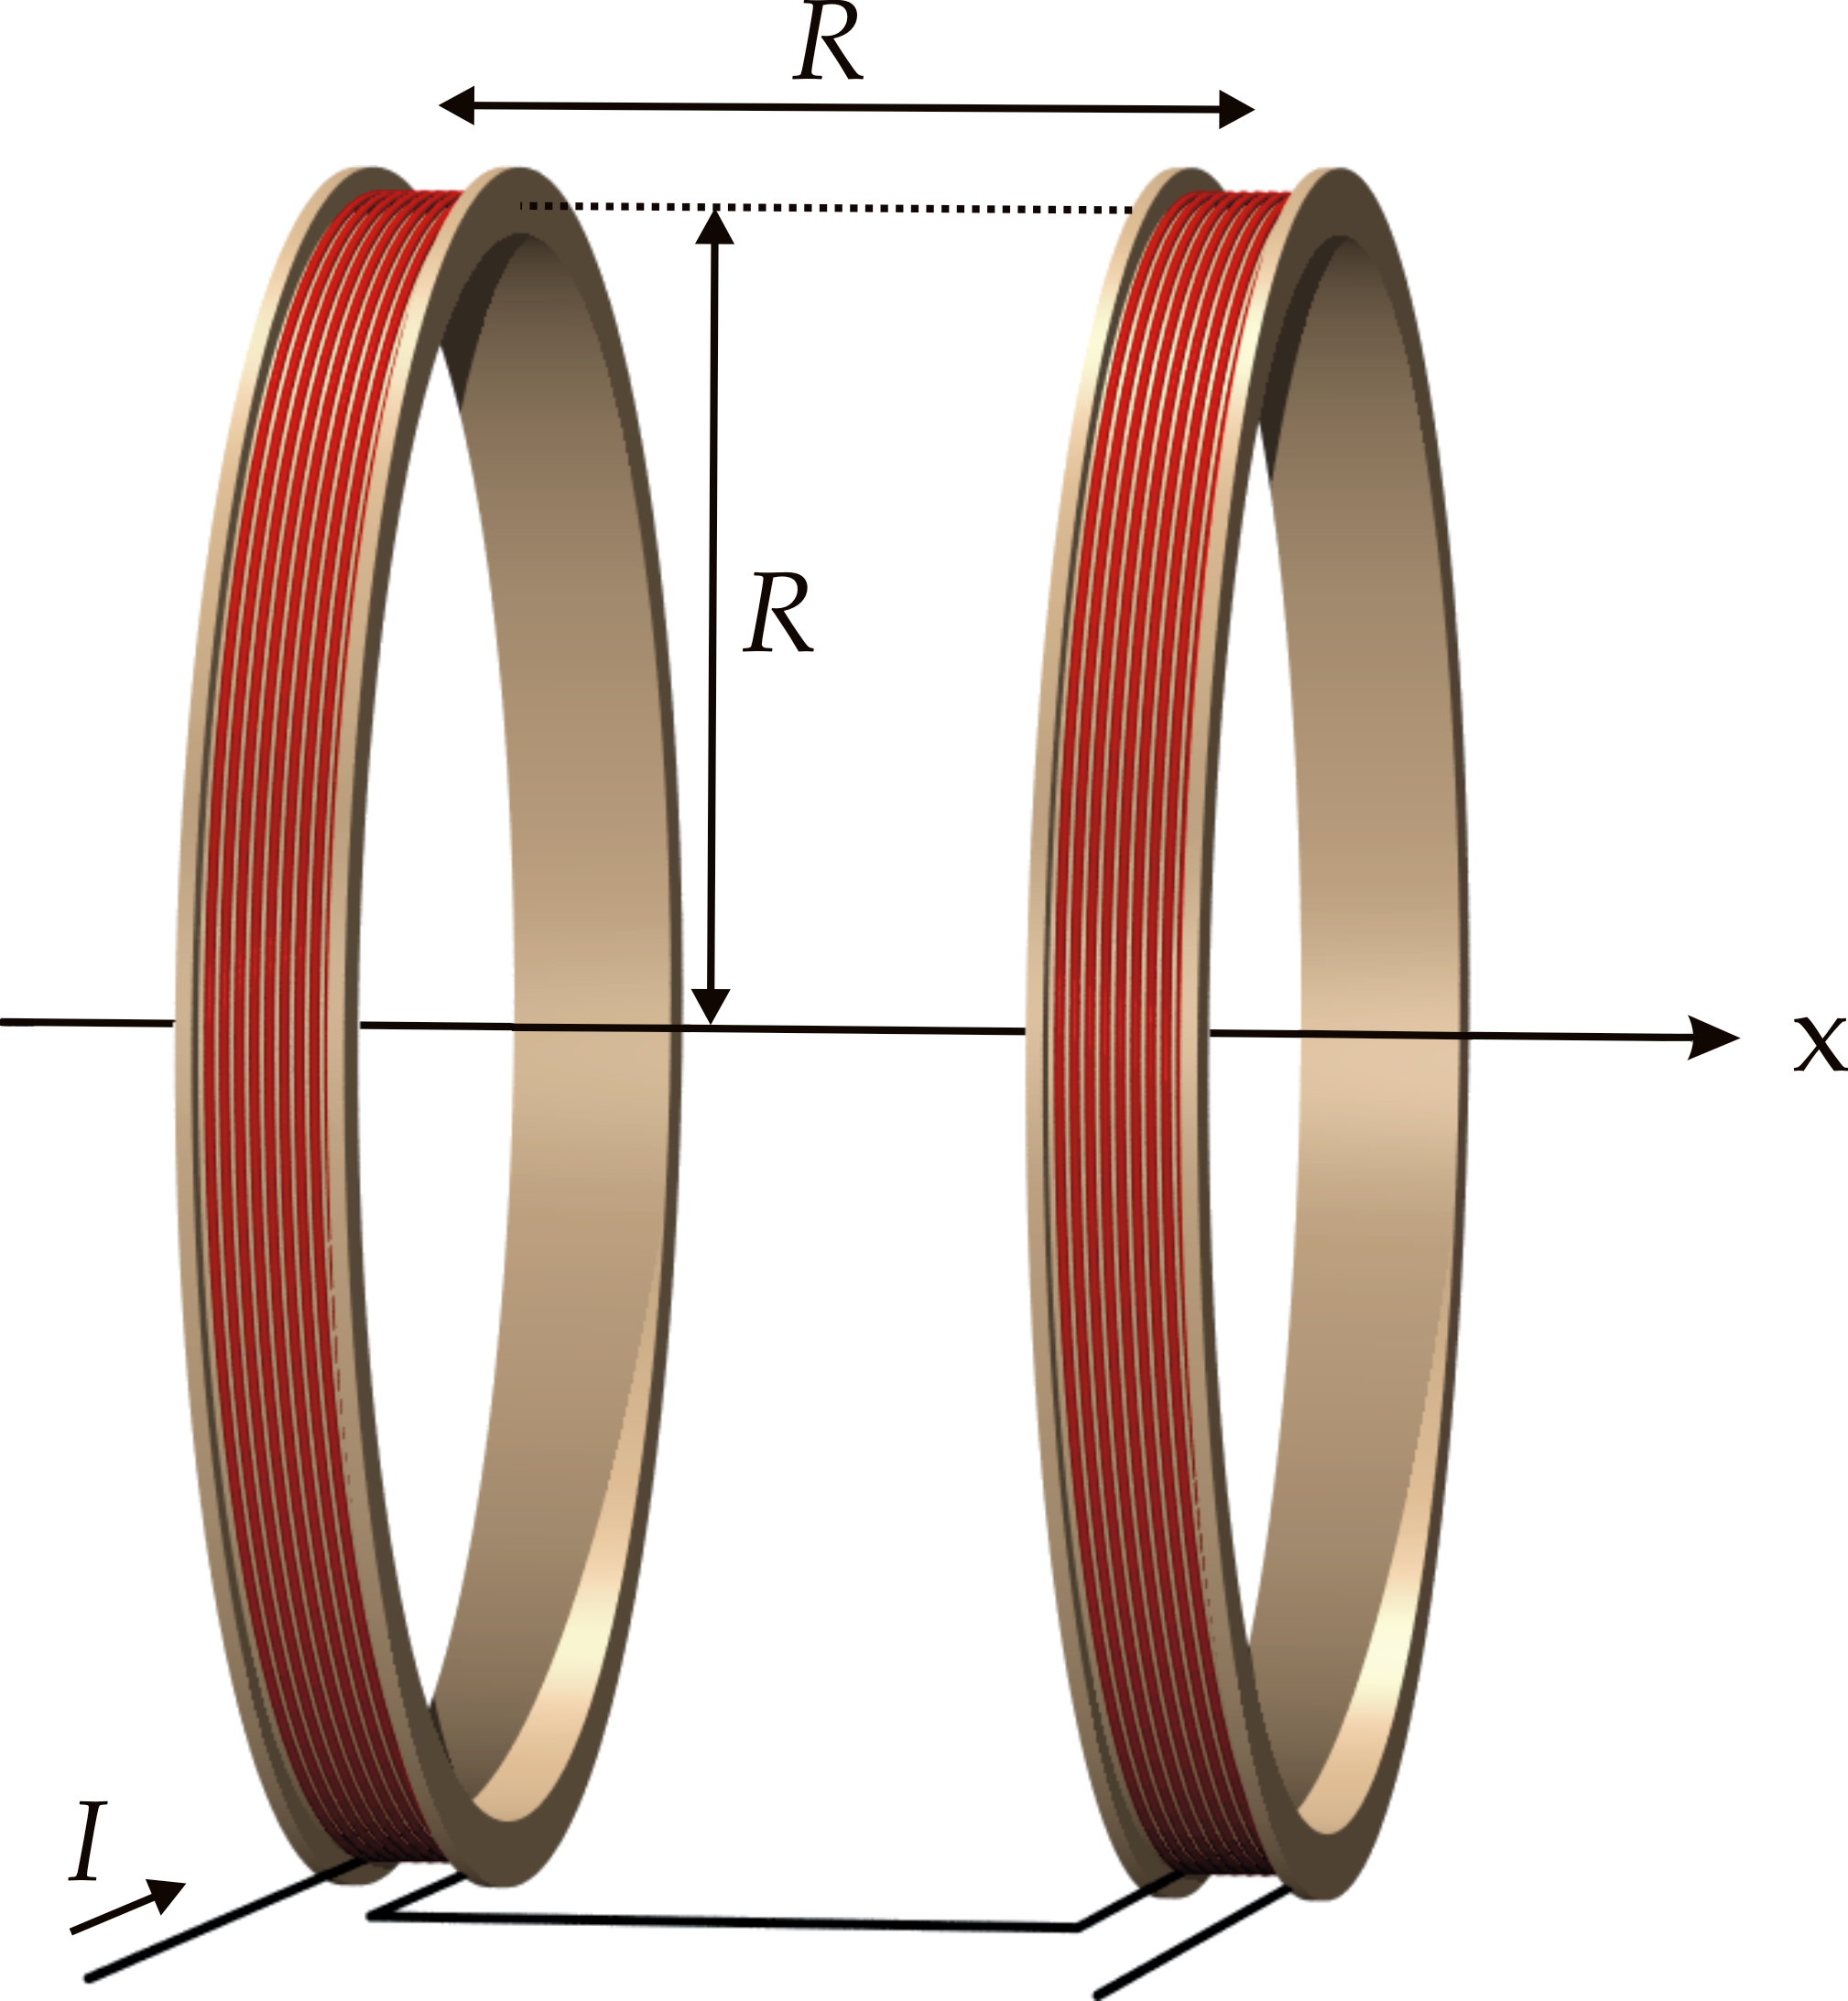
\includegraphics[width=5cm]{helmholtzspule.png}
\caption{Aufbau einer Elektronenkanone} \label{elektronenkanone}
\end{figure}

Die Helmholtzspule ist eine Apparatur zur Erzeugung eines homogenen Magnetfeldes. Das wird erreicht, indem zwei (kurze) Leiterschleifen vom Radius $R$ parallel zueinander von einem Strom durchflossen werden. Die zwei Spulen erzeugen jeweils ein inhomogenes Magnetfeld, welche sich aber so überschneiden, dass auf der Geraden durch beide Leitermittelpunkte ($\hat{e}_x$-Achse) ein (in guter Näherung) homogenes Magnetfeld entsteht. Für dieses Magnetfeld ergibt sich durch Symmetrie nur eine Abhängigkeit von der $\hat{e}_z$-Achse, sodass sich das Magnetfeld ergibt zu:
%\begin{align}
%B_{z} & = \frac{1}{2} \mu_{0} \mu_{r} n I R^2 \left[ \left( R^2+ %\left( z - \frac{R}{2} \right)^2 \right)^{- \frac{3}{2}} + \left( R^2 + \left( z + \frac{R}{2} \right)^2 \right)^{- \frac{3}{2}} \right] \text{.} 
%\end{align}
\begin{align}
B&=\frac{8}{\sqrt{125}}\mu_0\mu_r\frac{nI}{R} \label{helm}
\end{align}

\subsection{Bestimmung des Quotienten $\frac{e}{m_e}$}
Zur Herleitung des Quotienten $\frac{e}{m_e}$ kann man das Kräftegleichgewicht betrachten. Dazu werden folgende zwei Kräfte betrachtet:
\begin{itemize}
\item Lorentzkraft $\vec{F}_L$
\item Zentripetalkraft $\vec{F}_Z$
\end{itemize}
Die Lorentzkraft ist die Kraft, die auf ein Elektron in einem $\vec{E}$- oder $\vec{B}$-Feld wirkt:
\begin{align*}
\vec{F}_L&=q\left(\vec{E}+\vec{v}\times\vec{B}\right)\text{.}
\end{align*}
Da wir bei unserem Experiment nur ein Magnetfeld betrachten, also $\vec{E}=0$, lässt sich die Lorentzkraft auch schreiben als:
\begin{align}
\vec{F}_L&=q\vec{v}\times\vec{B}.
\end{align}
Die Zentripetalkraft $F_Z$ hingegen ist die Kraft, die auf einen um einen festen Punkt rotierenden Körper wirkt:
\begin{align}
\vec{F}_Z&=\frac{m_ev^2}{r}\text{.}
\end{align}
In unserem Fall sind beide Kräfte gleich, wenn das Elektron im $\vec{B}$-Feld im Kreis rotiert. In diesem Fall lässt sich der für
unser Experiment gesuchter Radius $r$ bestimmen.

\begin{align}
F_Z&=F_L \\
\frac{m_ev^2}{r}&=q\vec{v} \times \vec{B} \\
\Rightarrow \frac{e}{m_e}&=\frac{v}{Br}
\end{align}
Durch Einsetzen des Magnetfeldes ergibt sich für den Quotienten $\frac{e}{m_e}$:
\begin{align}
\frac{e}{m_e}&=\frac{125U_BR^2}{32\left(r\mu_0\mu_rnI\right)^2}\text{.}
\end{align}

\subsection{Elektronenstrahl}
In diesem Versuch ist ein Elektronenstrahl sichtbar und wird abhängig vom Magnetfeld abgelenkt. Wir können diese Elektronen selber nicht direkt sehen, die Elektronen regen aber beim Zusammenstoßen mit Gasmolekülen diese an, sodass sie beim Zurückgehen in den Ausgangszustand Energie in Form von Licht abstrahlen. 